\documentclass[12pt]{article}

\usepackage[top=1.0in, bottom=1.0in, left=1.0in, right=1.0in]{geometry}
%\pagenumbering{gobble}

\usepackage{graphicx}
\graphicspath{ {./images/} }

\title{CS221 Research Project Report\\Closed Path Rollercoaster Track Generation\\using Motion Planning Search}
\date{Winter 2021}
\author{Terrell Ibanez}

\begin{document}
\maketitle{}

\section*{Introduction}
Rollercoasters are an interesting version of the motion planning problem - while real world constraints like financial cost do apply, instead of the shortest or most efficient path, a coaster should be ``taking the scenic route'' so to speak.

However, unlike a path winding through a park where a route being scenic is defined by the trees and various stationary objects, the interesting-ness of the path itself is what matters.

\section*{Literature Review}
Upon examination, the generation of rollercoasters using artifical intelligence is a particularly interesting problem because it has not been well studied academically.
I was unable to find any published papers relating to the generation of coasters using artificial intelligence, but there have been other attempts informally.

The primary work looked at was Dylan Ebert's Neural RCT, a sequence-to-sequence (Seq2Seq) Long Short-Term Memory (LSTM) model trained with wooden rollercoaster tracks for Rollercoaster Tycoon 2 (RCT2), a nearly two decade old classic video game from 2002.

Documented in Ebert's work are difficulties with dealing with RCT2's Run Length Encoding (RLE), which the original author, Chris Sawyer, used to save space by compressing repeating runs of the same byte (mostly zeros), as tracks were of a fixed length when decoded.
Ebert's decoder attempts to load the track while decoding at the same time, leading to track loading failures on about half of the tracks used.
Ebert's track generator does not directly make the RCT2 track files, it gives track pieces for a user to input into RCT2.
I suspect this to be primarily due to the RLE difficulties.

Aside from the difficulties of dealing with a game this old, in the end, the primary issue with his approach is that Seq2Seq models don't consider / attempt to close the loop. He suggests that humans using his track generation tool do so manually.
Another rollercoaster generation project - an Art of Engineeering video about generating coaster curves also shares this same issue (though primarily as it's 2-dimensional).
\section*{Dataset}
The original approach to the dataset was to follow Dylan Ebert, and use coasters built / published by the general public.
While I did spend a great amount of time making my own track decoder to deal with RCT2's RLE that works properly, it became apparent that also using a Seq2Seq approach would just lead to the same problem of not finishing the coaster.
As a result, the task was reformulated as a motion planning search problem, as described later.

\section*{Baseline}
The original baseline selected were the coasters generated by Dylan Ebert's approach, in that his coasters do not form a closed path, but tend to be varied / interesting.
Unfortunately his code was written some time ago and no longer runs properly in Tensorflow due to deprecated APIs.
However he does provide some screenshots of his generated coasters, which is enough for a rough visual comparison - those tracks that can be viewed on his site in the references.
\section*{Main Approach}
The main approach to solving the generation problem was to shift focus from a sequence to sequence model re-thinking it as a motion planning search problem.

To pose this task as a motion planning problem, consider the coaster car to be an agent that moves through 3D space, with state to be the current orientation of the coaster car, and available actions to be track piece selections that alter that state.
The sequence of track selections while searching to get the car to the station then forms the coaster track path.

To simplify the problem, because every coaster has a station and (most) coasters need at least one lift hill to build up potential energy, the track starts with a station and an initial spiral lift hill.
The state is simulated from the initial state in the station up through the lift-hill, making the starting state for the search the top of the spiral lift hill, and the goal for the motion planning to have the coaster state at the return entrance of the station.

To generate possible track selections during the search, a state machine with valid paths was constructed where certain transitions to new states are only possible based on the current state.
As an example, a track cannot go directly into a left roll from a right roll, it must transition into a level state and then go into a left roll. This applies similarly to up or down slope.

After track possibilities are generated, those are validated against height build limits and self-intersection. The self intersection validation works by generating a set of volumetric collider 3D grid points for a given track sequence, as well as a set of points for a potential track.
The track piece collider points are then inserted into the set - if any of them already exist it collides in 3D space, or is too close for minmimum safe distances.

\section*{Evaluation Metric}
The initial primary evaluation metric was to see if the coasters generated are closed paths. Additionally it was important that the coaster be physically feasible, which imposed height and self-intersection limits . Visual interest of the coaster was also given small consideration.
\section*{Results \& Analysis}
\begin{figure}[h]
    \caption{Constant Cost Coaster in OpenRCT2}
    \centering
    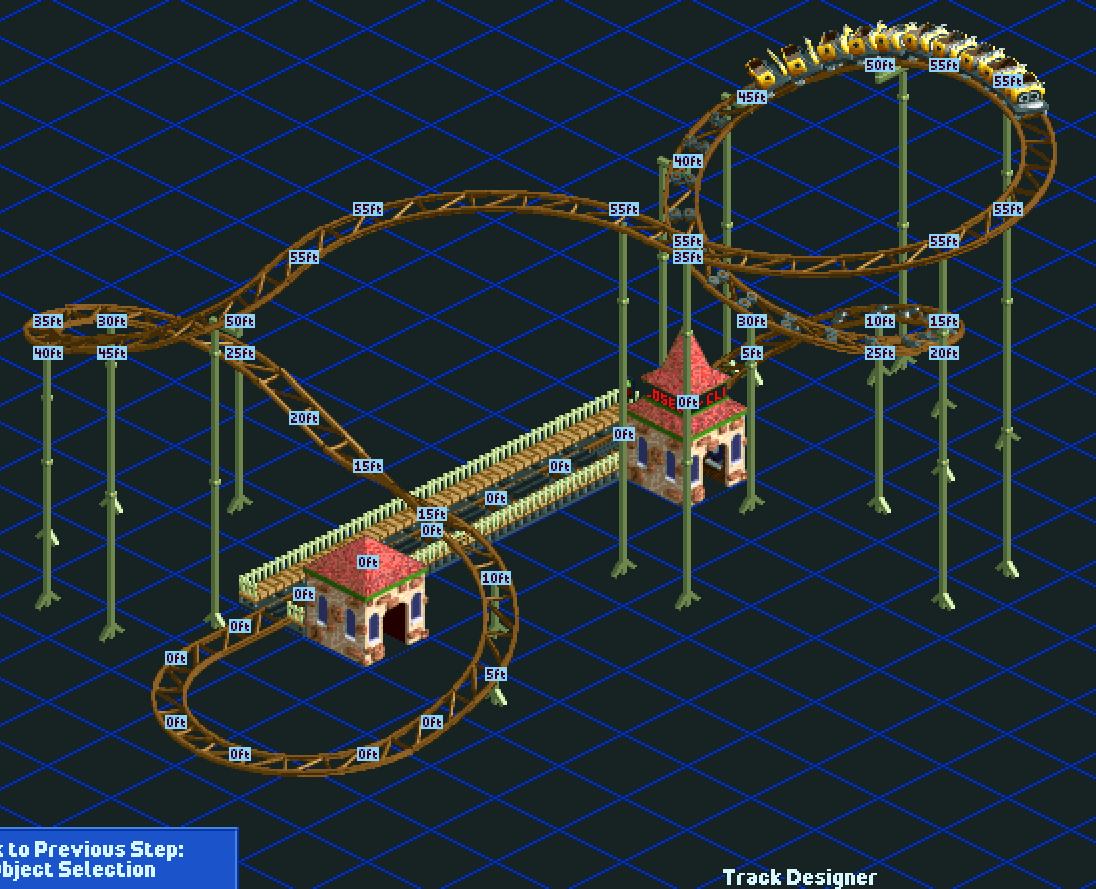
\includegraphics[width=0.75\textwidth]{coaster_constantcost}
\end{figure}

\begin{figure}[h]
    \caption{Constant Cost Coaster Collider Visualization}
    \centering
    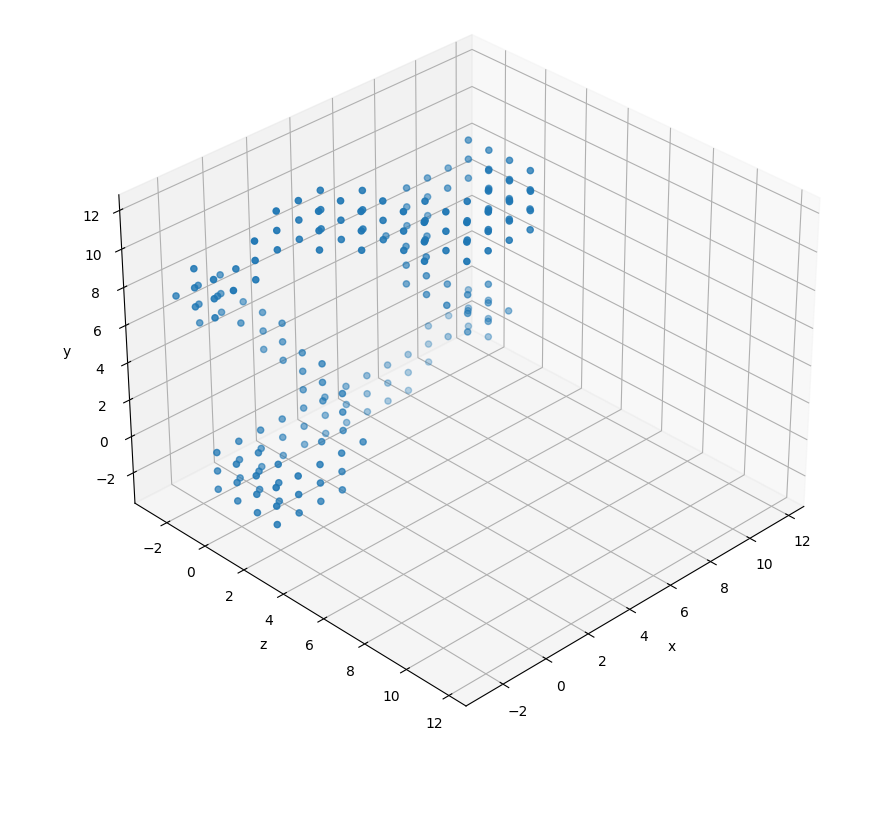
\includegraphics[width=0.75\textwidth]{collider_constantcost}
\end{figure}

\begin{figure}[h]
    \caption{Financial Cost Coaster in OpenRCT2}
    \centering
    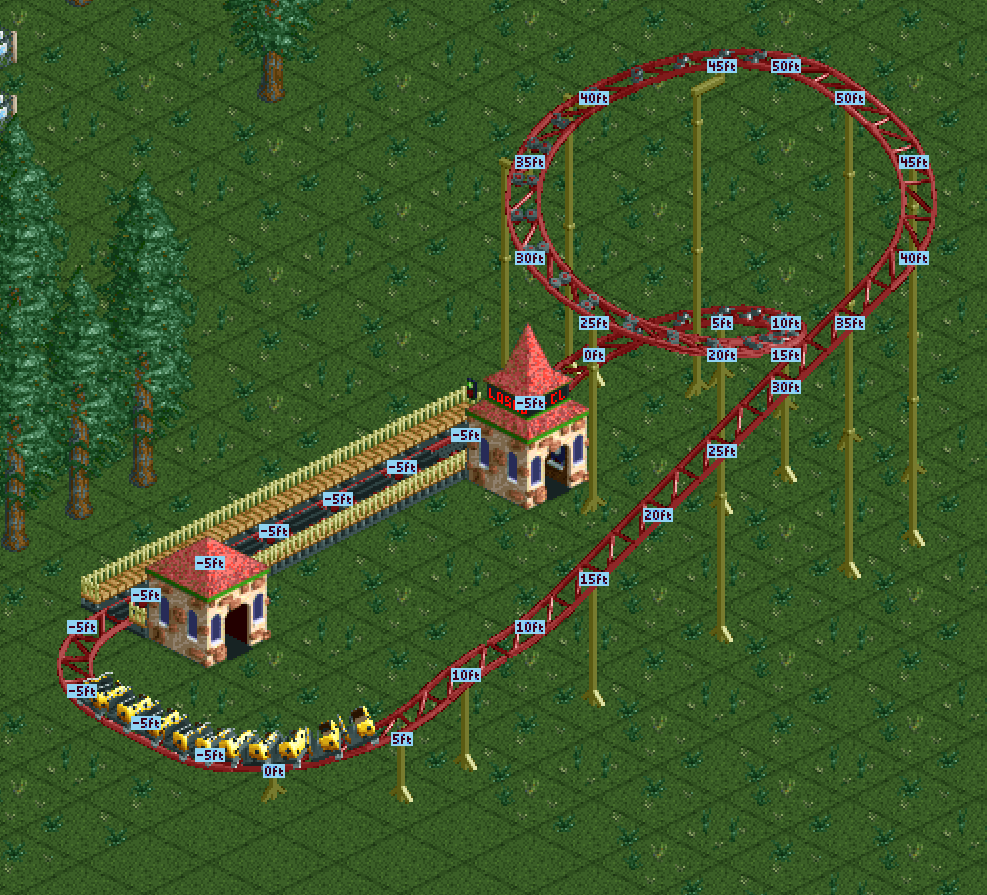
\includegraphics[width=0.75\textwidth]{coaster_financialcost}
\end{figure}

\begin{figure}[h]
    \caption{Constant Financial Cost Coaster Collider Visualization}
    \centering
    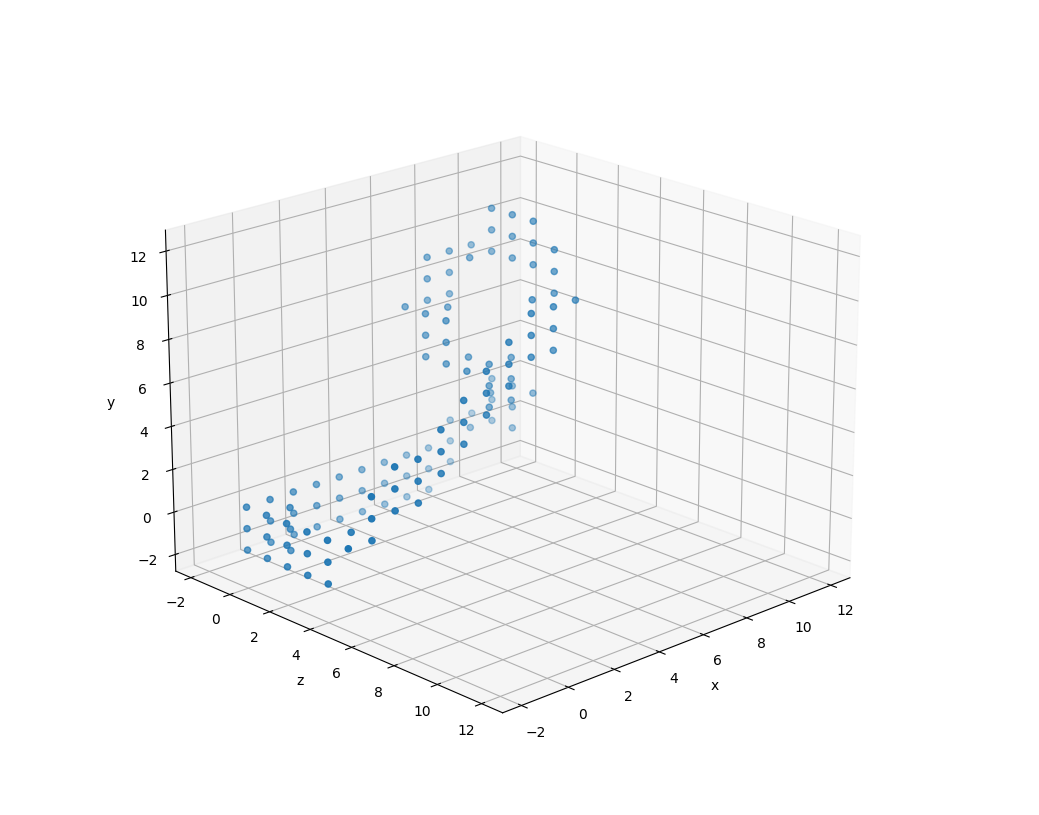
\includegraphics[width=0.75\textwidth]{collider_financialcost}
\end{figure}

The initial result using A* with a constant cost for track pieces worked surprisingly well - but when trying to build the track in OpenRCT2 I discovered that while it did complete the path, it did so by placing track pieces through itself.

This was fixed by adding the volumetric collision detection as described earlier, and the results of that are shown in Figures 1 and 2.

When adding in the ability for the A* search to consider the costs of the track pieces, it makes a much less interesting coaster as demonstrated in Figures 3 and 4.
I suspect this is due to more "interesting" rollercoaster track pieces being more expensive than regular pieces.

However, compared to Ebert's coasters (which can be viewed on his site) these coasters are much less interesting visually, and possess a lot less variety.

It's very clear from the results that something needs to be added to make the coasters more interesting, and potential approaches on that are described in the future work section.

\section*{Future Work}
To solve the major potential safety issues with the coasters the search algorithm creates, it would be necessary to simulate (or at least approximate) the physics state of the coaster car.
With a physics implementation it would be possible to automatically check / verify safety constraints, such as imposing a negative penalty to cost for high-G turns that are not banked, or if a design leads to a coaster state with too much / not enough kinetic energy.

Additionally, with the implementation of physics, it would be possible to write the search problem to also create the station and the lift hill by imposing an incentive or cost discount to the search for building up potential energy early on.

One of the issues with posing it as a search problem is that the AI will pick the same path each time.
A potential approach to solving that issue would be to borrow from the approaches of Generative Adversarial Networks and perform a "Generative Adversarial Search".
Using the existing collision checking system, one could have an adversary (semi-randomly) add blockers that force the path search to take a longer / more varied (and hopefully more interesting) path.

\section*{Code}
The code is available on GitHub:\\
https://github.com/ibnzterrell/RCTMotion

\begin{thebibliography}{9}
    \bibitem{TD6}
    James Hughes. RCTTech Depot Archive - TD6 File Format\\
    https://freerct.github.io/RCTTechDepot-Archive/TD6.html

    \bibitem{DEbert}
    Dylan Ebert. Neural RCT\\
    https://dylanebert.com/neural\_rct/

    \bibitem{ArtEngAI}
    Art of Engineering. Can A.I. Design the Perfect Roller Coaster?\\
    \texttt{https://www.youtube.com/watch?v=4l5MGqrAItU}
\end{thebibliography}
\end{document}